\label{condi}
\section{The Sensors} 

The sensors used in this project are microfabricated on a single silicon chip, and kindly provided by professor Dr. Sandro Carrara research group from  \'{E}cole
Polytechnique F\'{e}d\'{e}rale de Lausanne (\textit{EPFL}), Switzerland.


The choice of using a microfabricated sensor instead of a commercial one (the number of commercial sensors is very high even for biomedical applications) has been taken because of a remarkably decrease in sensing occupied space. Indeed, in this way, the area consumption can be optimized.

\begin{figure}[h]
	\centering
	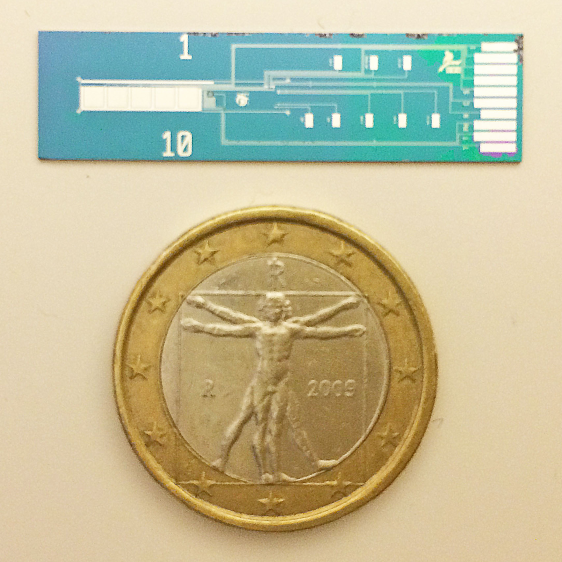
\includegraphics[scale = .4]{Sensors/multisensor}
	\caption{Multisensor - Size Comparison}
	\label{Fig:mulsize}
	
\end{figure}

The (Fig.\ref{Fig:mulsize}) shows the sensor and highlights its very small dimension ($35.1\ x\ 9.3\ mm$). This multisensor contains an Iridium Oxide based pH sensor and a platinum resistance temperature detector (\textit{RTD}) \cite{DFTSA}.\\
The device also hosts five independent working electrodes (\textit{WE}), with shared platinum reference electrode (\textit{RE}) and platinum counter electrode (\textit{CE}). But, at least for the time being, we are not going to use them.

The (Fig.\ref{Fig:mulsensor}) shows the circuit schematic of multisensor. As can be seen, from the interface the pads that are going to be used in this thesis are the four on the bottom. In fact,  the last pair of pins are the temperature ones, and the penultimate ones are tied to the pH sensor (negative pin on top).
 
 \begin{figure}[h]
 	\centering
 	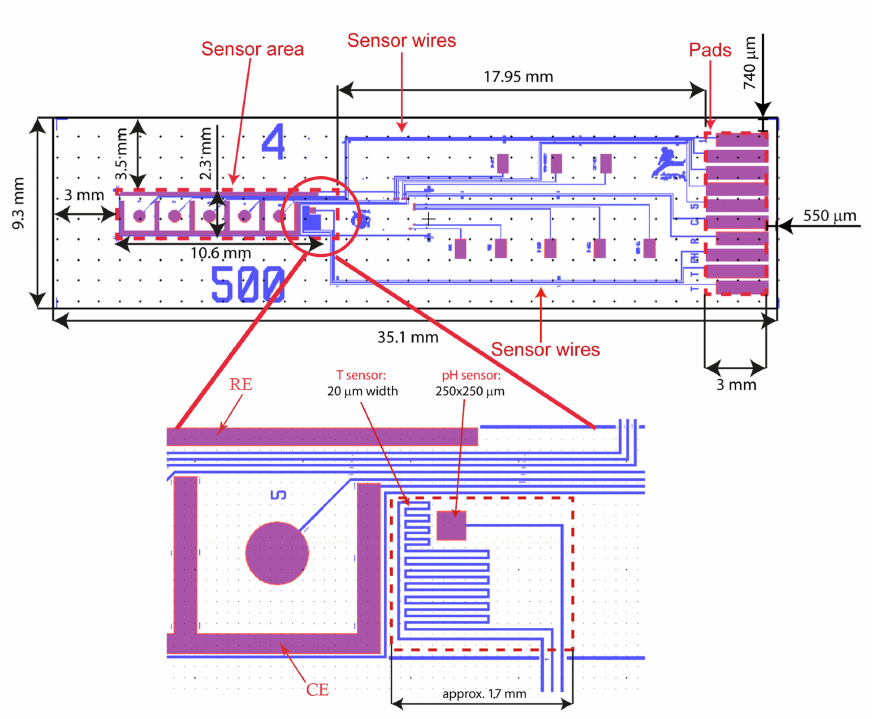
\includegraphics[scale = .5]{Sensors/multisensor1}
 	\caption{Multisensor - Scheme}
 	\label{Fig:mulsensor}
 	
 \end{figure}
 
 \subsection{PH Sensor}\label{sec:sensorPH}
 
 The embedded pH sensor has been made by platinum. Its electrical output is a voltage value which varies almost linearly with the pH.
 
 The pH sensor needs to be calibrated before it can be used. The calibration and characterization of sensor are made in different environments and with different solutions. After this step the transfer function of the sensor is linear (Fig.\ref{Fig:typicalph}) with a slope of around $- 100\ mV/pH$.
 \subsection{Temperature Sensor}\label{sec:sensorT}
 
 For almost all the metal materials, electrical resistance is a parameter which varies with temperature. In order to create a resistance temperature detector (\textit{RTD}), a coupled system of a metal wire and a resistance measurement device is needed. Inside the used device, the temperature sensor is made by a platinum wire. This metal is strongly used for temperature applications because it allows to obtain the most accurate measurements (up to $\pm 0.001\ \text{°}C$) with a linear output response.
 
 The relationship between resistance and temperature of a platinum resistance thermometers is described by the \textit{\textbf{Callendar-Van Dusen}} equation (Eq.\ref{Eq:vancosa}).
 
 \begin{equation}
 R\left(T\right) \text{ = } R\left(0\right) \cdot \left[1 \text{\textit{+}} A\cdot T \text{\textit{+}} B \cdot T^2 \text{\textit{+}} \left(T-100\right)\cdot C \cdot T^3\right]  \label{Eq:vancosa} \end{equation}
 
 Where:
 \begin{itemize}
 	\item $R\left(T\right)$, is the resistance at the $T$ temperature;
 	\item $R\left(0\right)$, is the resistance value at $0\ \text{°}\ C$;
 	\item $A$, $B$, and $C$, are the \textit{Callendar-Van Dusen constants} defined by the following:\begin{subequations} \begin{align} 	A &\text{ = }\alpha \text{+} \frac{\alpha\cdot\delta}{100},\\B &\text{ = } - \frac{\alpha\cdot\delta}{100^2},\\ 	C &\text{ = } - \frac{\alpha\cdot\beta}{100^4}. \end{align} \end{subequations}
 \end{itemize}

And $\alpha \text{ = } 0.003921 \varOmega/\text{\textdegree}C$, $\beta  \text{ = } 0$ for positive temperature and $\delta  \text{ = } 1.49$.

 
 \begin{figure}[h]
 	\centering
 	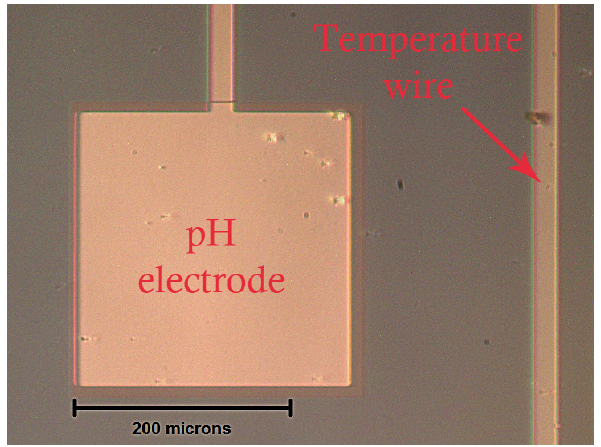
\includegraphics[scale = .5]{Sensors/multi}
 	\caption{PH and Temperature Sensors from an Optical Image}
 	\label{Fig:close}
 	
 \end{figure}
 
 The pH and temperature sensors are very close from each others (Fig.\ref{Fig:close}), and this is very important because the pH electrode's sensitivity varies over temperature, thus: temperature affects the pH value, as can be seen from (Eq.\ref{eq:pH}). So, we always need to know at what temperature  we make the pH measure.
 
 \begin{equation}
 pH\left(X\right) \text{ = } pH\left(S\right) \text{\textit{+}} \frac{\left(E_S - E_X\right) \cdot F}{R \cdot T \cdot \ln\left(10 \right)} 
 \label{eq:pH}
 \end{equation}
 
 The (Eq.\ref{eq:pH}) represents the transfer function of a pH sensor, where:
 \begin{itemize}
 	\item $pH\left(X\right)$, is the pH value of unknown solution;
 	\item $pH\left(S\right)$, is the pH value of standard solution ($7$);
 	\item $E_S$, is the electric potential at standard electrode;
 	\item $E_X$, is the electric potential at pH-measuring electrode;
 	\item $F$, is the Faraday constant ($9.6485309\cdot10^4\ C\ mol^{-1}$);
 	\item $R$, is the universal gas constant ($8.314510\ J\ K^{-1}\ mol^{-1}$);
 	\item $T$, is the temperature in Kelvin.
 \end{itemize}
 
 
 
 
\section{PH Conditioning}\label{phcon}

\label{sec:circuitPH}
As already explained in (Sec.\ref{sec:sensorPH}), the pH sensor is a passive sensor, which means no excitation source is required because the sensor itself generates its own electrical output signal. In particular any variation of pH in input is transduced in a voltage variation in output.\\

The pH sensor is also bipolar, this means the voltage output may be both positive and negative, as shown in (Fig.\ref{Fig:typicalph}).\\

\begin{figure}[h]
	\centering
	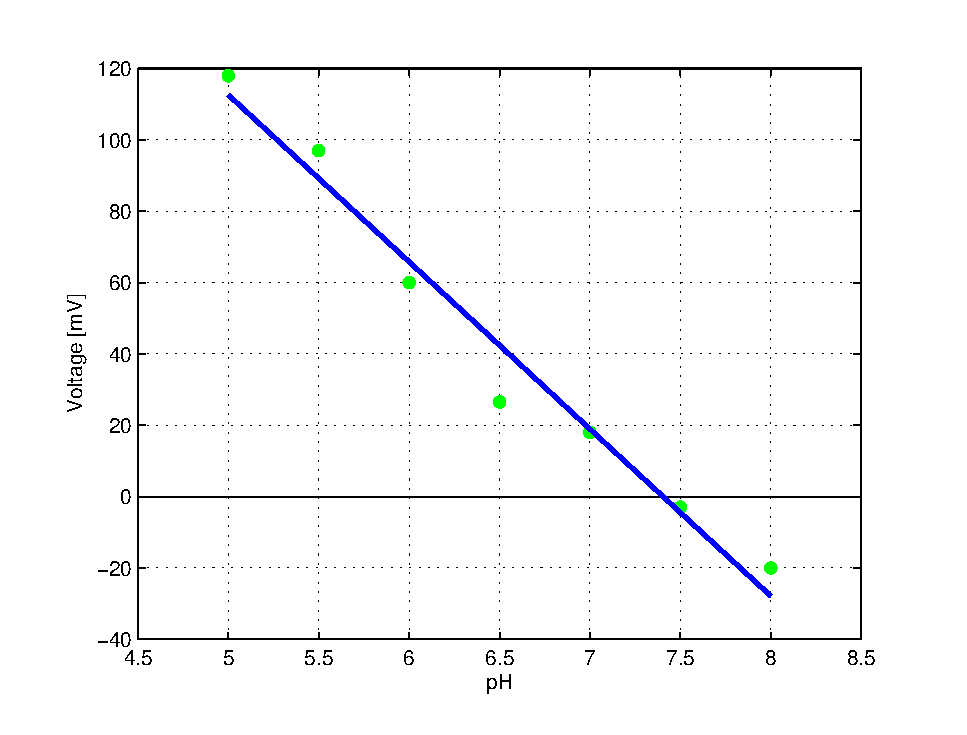
\includegraphics[scale = .65]{Sensors/tipicalph.eps}
	\caption{Typical pH-sensor transfer function}
	\label{Fig:typicalph}
	
\end{figure}

Resuming, it produce a voltage output that decreases linearly with pH of the solution being measured. The sensors give a sensitivity which ranges between $50$ and $120$ $mV/pH$ (it depends from sensor to sensor), this means that, in order to well observe this variation, an amplification stage may be required.

The (Fig.\ref{Fig:circuitph}) shows the adopted solution for conditioning the pH sensor. \\
Fist of all, since the pH sensor produces a bipolar signal and this application operates on a single voltage supply, the signal has been level shifted. To achieve this first challenge the operation amplifier \textit{U1} forces an off-set of $512\ mV$ to the pH sensor. Indeed, the \textit{LM4140A-1.0} is a high precision low noise \textit{LDO} (Low Drop Out) voltage reference which provides an accurate $1.024\ V$. This voltage has been halved by the $10\ K\Omega$ resistor divider. The \textit{U1} is in voltage follower configuration, thus its output should be equal to the input, and it biases the reference electrode of the pH sensor with $512\ mV$, at low impedance.\\
So, what the part of circuit made by \textit{U1} and \textit{LM4140A-1.0} does is to shift the bipolar pH sensor signal to an unipolar in order to be usable in the single-supply system.
 
\begin{figure}[h]
	\centering
	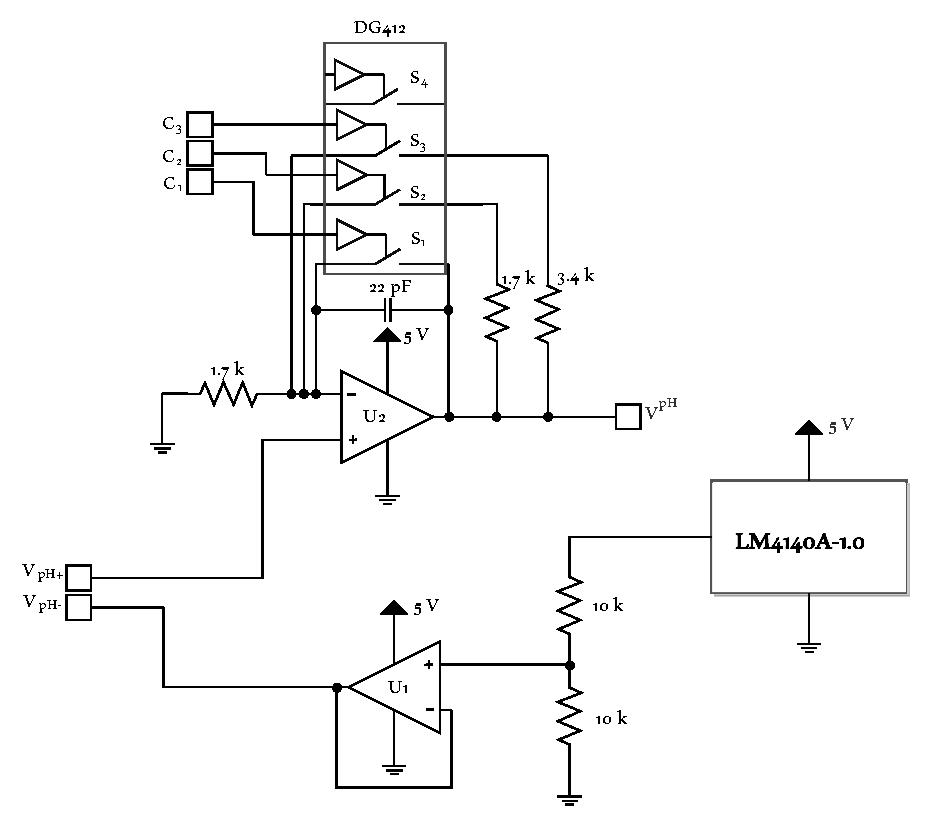
\includegraphics[width=\textwidth]{Sensors/phCircuit.eps}
	\caption{Conditioning circuit for pH sensor}
	\label{Fig:circuitph}
	
\end{figure}

Another challenge is given by the high impedance of the electrode. In fact the output impedance of the pH sensor is higher than $100\ M\Omega$. The circuit in (Fig.\ref{Fig:high}) shows a typical connection of this sensor where the output voltage is given by:

\begin{equation}
V_{out} \simeq V_{in} \text{ \textit{=} } V_{S} - I_{bias} \cdot R_{S}
\end{equation}

Thus, in order to reduce the error caused due to amplifier's input bias current a really low input bias current amplifier has to be chosen. For this reason, the 
\textit{LMP7721} is used, it is has an ultra-low input bias current ($3 \pm 17\ fA$).\\


\begin{figure}[h]
	\centering
	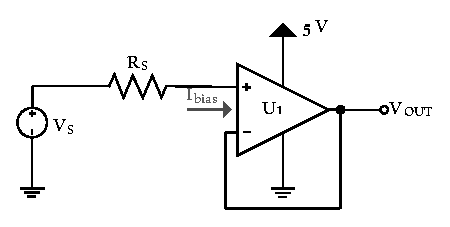
\includegraphics[]{Sensors/highimpedence.eps}
	\caption{Error caused by Amplifier's Input Bias Current}
	\label{Fig:high}
	
\end{figure}

In (Fig.\ref{Fig:circuitph}) both \textit{U1} an \textit{U2} are \textit{LMP7721}. The second amplifier with the \textit{DG412} represents a simple \textbf{PGA} (\textit{Programmable Gain Amplifier}), where the resistors have been chosen to give the following gains:
\begin{itemize}
	\item $1$, when $C_1$ is asserted and the others are denied;
	\item $2$, when $C_2$ is asserted and the others are denied;
	\item $4$, when $C_3$ is asserted and the others are denied.
\end{itemize}

The feedback capacitor is used to ensure stability and holds the output voltage during the switching times. Indeed, in these slice of time the output node would be floated without the capacitor.\\
This PGA stage introduces an additional offset error of  $75 \pm 470\ fV$, due to the bias current of the operational amplifier and $R_{ON}$ of \textit{DG412} ($25\ \varOmega$). That voltage combined with the \textit{LMP7721} offset (which is very higher than the first one) is approximately equal to $26\ \mu V$.\\

Since the environment in which the circuit is going to be used is a laboratory, so a really noisy place, the conditioning circuit for the sensor has to involve the design of a \textit{\textbf{low-pass filter}} in order to reject the noise.\\

The circuit shown in (Fig.\ref{Fig:filterCircuit}) is a third order low-pass filter with a \textit{Bessel} response. It has been designed in order to ensure a really flat-response in the pass band. \\
The parameter of the filter are:

\begin{enumerate}
	\item \textit{cutoff frequency} ($f_c$): $26.8\ Hz$, ;
\item \textit{stop band attenuation}: $-28.2\ dB$ at \textit{stop band frequency} ($f_s$) $60\ Hz$ (the line frequency in USA);
\item \textit{Quality factor} ($Q$): $0.65$;
\item \textit{filter order}: third;
\item \textit{filter response}: Bessel.
\end{enumerate}

It's important that $Q < 0.707$ because otherwise would be some peaking in the filter response. While, in this case, as shown in (Fig.\ref{Fig:filterbode}), roll-off at the cutoff frequency is greater.\\
This filter also behaves as \textit{anti-aliasing filter}, to prevent the aliasing components from being sampled during the analog to digital conversion.\\



\newpage
\clearpage

\begin{figure}[h]
	\begin{center}
	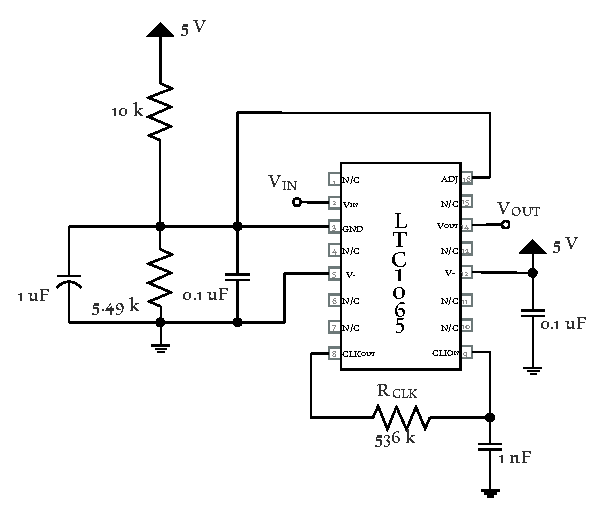
\includegraphics[height=.38\textheight]{Sensors/filterCircuit}
	\caption{Low-Pass Filter Schematic}
	\label{Fig:filterCircuit}

	\centering
	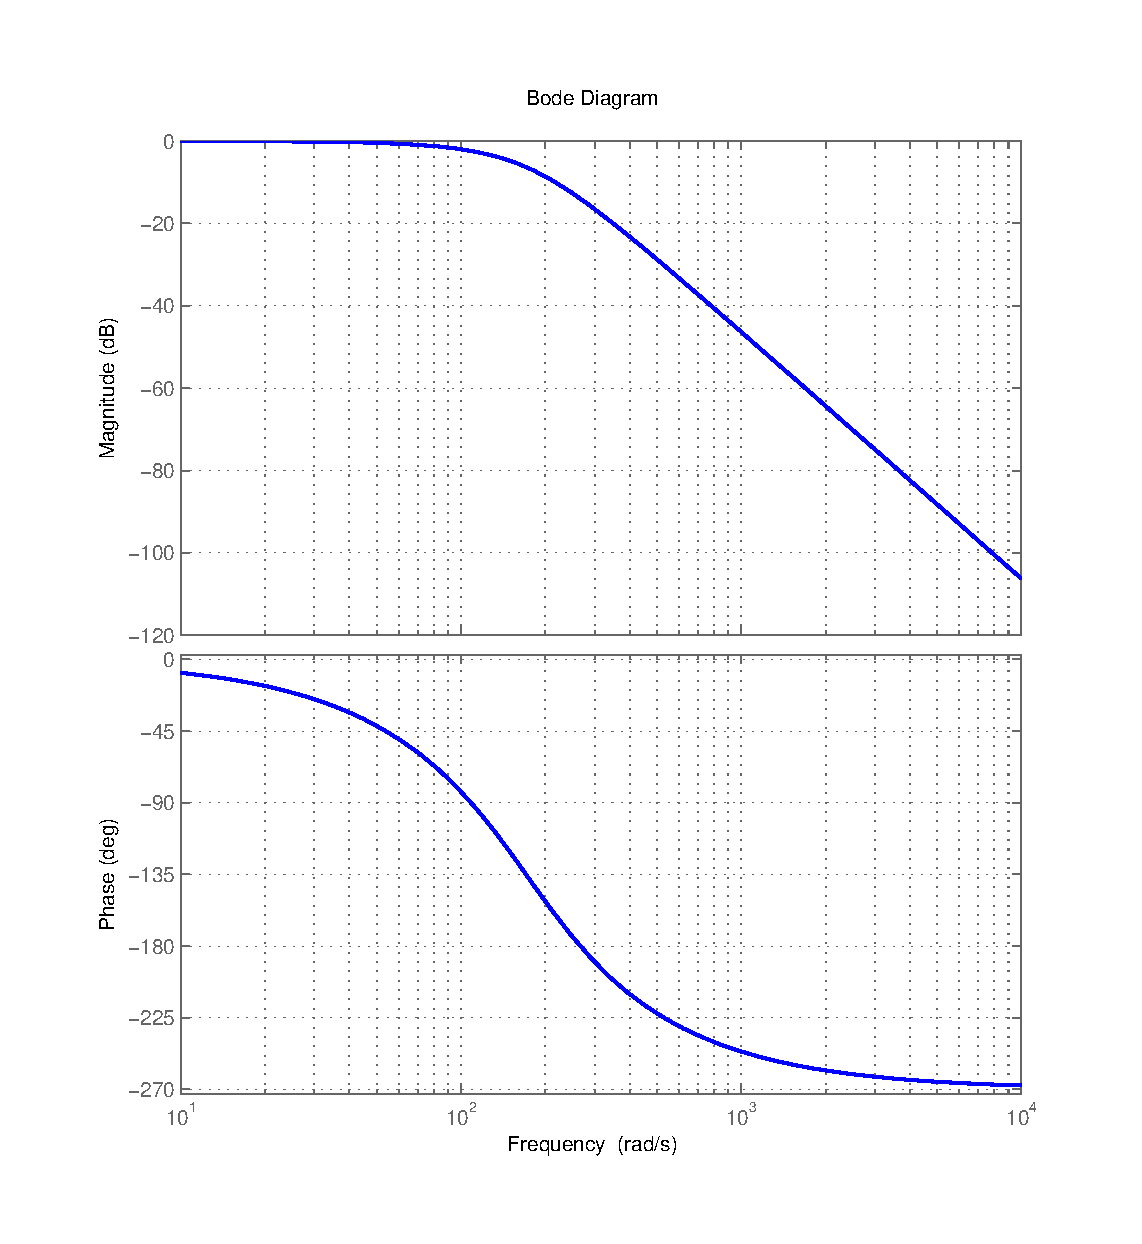
\includegraphics[height=.6\textheight]{Sensors/filterBode}
	\caption{Low-Pass Filter Frequency Response}
	\label{Fig:filterbode}
	\end{center}
\end{figure}
	
	\newpage
	\begin{figure}[t]
The output of this filter represent the input signal of the embedded ADC inside the Beaglebone Black.\\

Connecting together al this part we obtain the circuit in (Fig.\ref{Fig:pHConditioning}) where we can also see the general purpose input/output pin used to drive the \textit{PGA} and the analog input used for the pH sensor. As it is explained in (Chap.\ref{ch:firmware}) \texttt{AN\_2} is used to let the microcontroller know about the added offset.

\vspace{10mm}

\centering
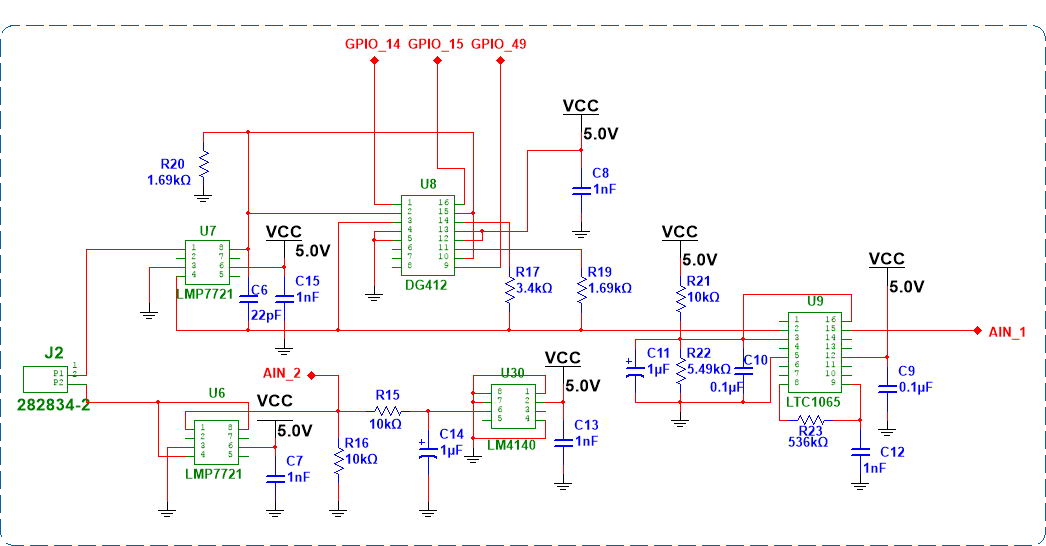
\includegraphics[width = \textwidth]{pcb/ph_conditioning}
\caption{Acquisition Path for pH Sensor}
\label{Fig:pHConditioning}
\end{figure}






\newpage
\clearpage

\section{Temperature Conditioning}\label{tempcon}



As already explained in (Sec.\ref{sec:sensorT}), the temperature sensor is a active sensor, which means excitation source is required because the sensor is resistor based so a current must be passed through it. Then, the corresponding voltage has to be measured in order to determine the temperature value.\\
So, any variation of temperature in input is transduced in a resistance variation in output.\\

The (Fig.\ref{Fig:temperatureCircuit}) shows the adopted solution for conditioning the temperature sensor.\\
In this connection the temperature sensor is excited by $680\ \mu A$, so the voltage $V_T$ is given by the following equation:

\begin{equation}
V_T \text{ \textit{=} } 680 \mu \cdot R_T
\end{equation}

\begin{figure}[h]
	\begin{center}
		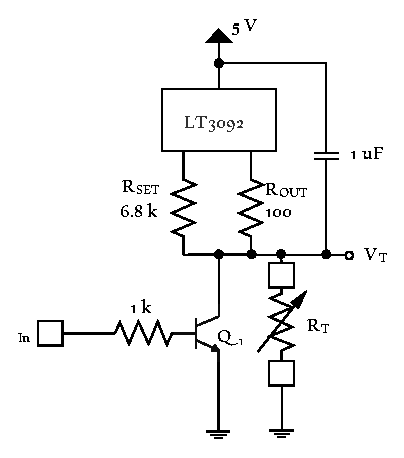
\includegraphics[height=.38\textheight]{Sensors/temperatureCircuit}
		\caption{Conditioning Circuit for Temperature Sensor}
		\label{Fig:temperatureCircuit}
	\end{center}
\end{figure}

In order to provide this amount of current a \textit{LT3092} is used. It can supply an output current equal to:

\begin{equation}
I_{OUT} \text{\textit{ = }} 10\mu \cdot \frac{R_{SET}}{R_{OUT}}
\end{equation}

To ensure the stability of the component, a feedback capacitor of $1\ \mu F$ is exploited. The transistor $Q_1$ is used to avoid the self-heating of the temperature sensor: when the temperature value has to be sampled $In$ is denied, for the remaining time $In$ is asserted, in this way the resistive sensor is by-passed, and the \textit{Joule} effect is avoided.\\

For the same reason exposed in (Sec.\ref{sec:circuitPH}), also in this case a filter is needed, and, since the voltage value is almost the same, the used filter is equivalent to the previous on.\\

\begin{figure}[h]
	\centering
	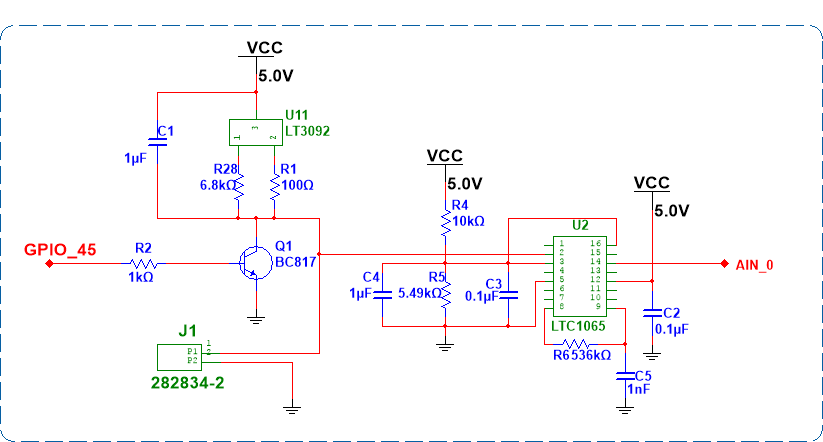
\includegraphics[width = \textwidth]{pcb/temperature_conditioning}
	\caption{Acquisition Path for pH Sensor}
	\label{Fig:temperatureConditioning}
\end{figure}

 
\section{Electrovalves Driver} \label{sec:electrovalves}

In order to allow the reverse control, from Google Glass to electrovalves, it is important to design a circuit that has to drive them from digital values provided by the \textit{Beaglebone Black} ($0$ equal to $0\ V$, $1$ equal to $3.3\ V$ and in both cases the maximum suppliable current is only $6\ mA$).\\

The electrovalves used are \href{http://www.festo.com/net/SupportPortal/Files/10026/MH1_VO_ENUS.pdf}{FESTO solenoid valves MH1}. They require a voltage of $24\ V$ in DC and a current of $80\ mA$.\\

\begin{figure}[h]
	\centering
	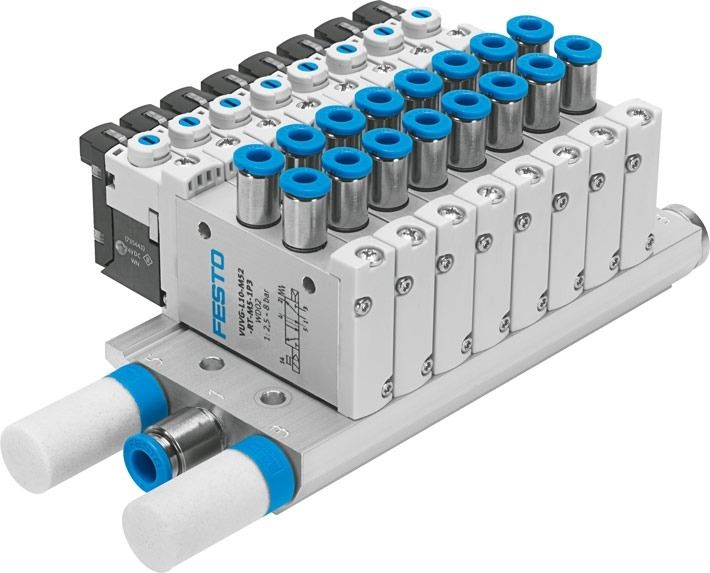
\includegraphics[width = .6\textwidth]{Driver/electrovalves}
	\caption{Electrovalves}
	\label{Fig:EV}
\end{figure}

To fulfill this aim a low-side switch MOS has been used, as shown in (Fig.\ref{Fig:driverEV}).

\begin{figure}[h]
	\centering
	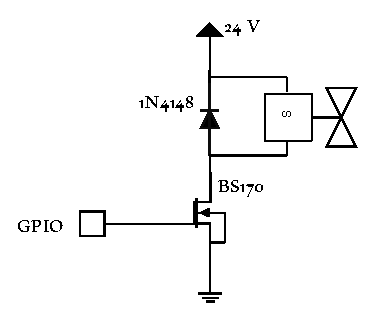
\includegraphics[]{Driver/driverEV}
	\caption{Driver for electrovalves}
	\label{Fig:driverEV}
\end{figure}

The \textit{Fairchild Semiconductor BS170 N-Chnnel MOS} has been chosen because of its low price and its capability of supporting a drain-source voltage of up to $60\ V$ and supplying a continuous drain current of up to $500\ mA$.\\

To protect the \textit{BS170} from reverse inductive current surges due to the solenoid of the electrovalve, a \textit{Vishay Semiconductors 1N4148 Diode} is used. It is able to support  a reverse voltage of up to $75\ V$ and a continuous forward current of up to $150\ mA$.\\

As shown in (Fig.\ref{Fig:EV}) the number of electrovalves used is eight, so the previous driver has been replicated in order to obtain the circuit in (Fig.)

\begin{figure}[h]
	\centering
	\includegraphics[width = \textwidth]{Driver/electrovalves_circuit}
	\caption{Electrovalves Driver Circuit}
	\label{Fig:electrovalves_circuit}
\end{figure}

\section{DC-DC Converter}

Since this system is supposed to drive different kind of electrovalves, which require a different value of voltage (but not in current) a \textit{DC-DC converter} is used in order to convert the voltage supply from $24\ V$ to $12\ V$. \\

Using the \textit{LT1374} the circuit in (Fig.\ref{Fig:DCDC}) has been designed, it is a constant frequency (equal to $500\ Hz$), current mode buck converter. It has an embedded clock and two feedback loops to control the duty cycle of power switch.\\
%This converter is able to supply a current of up to $2.5\ A$, that is definitely  bigger than the maximum required current, in which all the electrovalves are on in the same time: $80 \cdot 8 \text{ = } 640\ mA$.

\begin{figure}[h]
	\begin{center}
		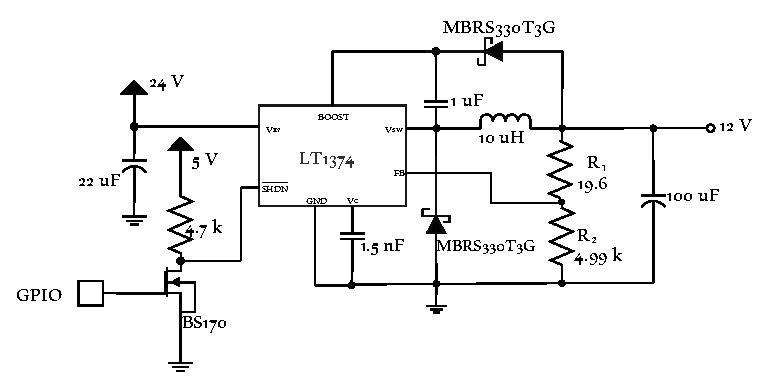
\includegraphics[width = \textwidth]{Sensors/dcdcCircuit}
		\caption{DC-DC circuit}
		\label{Fig:DCDC}
	\end{center}
\end{figure}

%The output capacitor not only behaviors like a low-pass filter in order to reduce the output spike, but it is used also to maintained the efficiency of \textit{DC-DC} over the output current range 

Trough a low-side switch, made with the \textit{BS170}, it is possible to shutdown the converter from the software. When the \textit{LT1374} is in shutdown, the supply current is reduced to $20\ \mu A$. As it is explained in (Chap.\ref{ch:firmware}) this is used to prevent regulator from operating when $24\ V$ are required.\\

\subsection{Components Choice}

All the components have been chosen with attention and for some reasons that are going to be explained belong.
\subsubsection{FEEDBACK RESISTORS}
The main behavior of the feedback pin on the \textit{LT1374} is to set the output voltage, and this deals with selecting the resistors $R_1$ and $R_2$. They are related from each others by the following equation:
\begin{equation}
R_1 = \frac{R_2 \cdot \left( V_{OUT} - 2.42\right)}{2.42}
\label{Eq:feedback}
\end{equation}
As suggested on datasheet of the component, the resistor between feedback pin and ground is $4.99\ k\varOmega$. So, from the (Eq.\ref{Eq:feedback}) results that the value of $R_1$ is $19.6\ k\varOmega$.
\subsubsection{INDUCTOR}
The choice of inductor is a trade-off among:
\begin{itemize}
	\item \textit{physical area}, lower values of inductor mean lower size;
	\item \textit{output current}, higher values of inductor allow more output current because they reduce peak current ($I_{SW\left(PEAK\right)} \propto 1/L$)
	\item \textit{ripple voltage}, higher values of inductor reduce the output ripple voltage.
\end{itemize}
A good choice is represented by $10\ \mu H$, with this inductor the maximum current peak (Eq.\ref{eq:peak}) is equal to $1.24\ A$.
\begin{equation}
I_{SW\left(PEAK\right)} \text{ = } I_{OUT} + \frac{V_{OUT \cdot \left(V_{IN} - V_{OUT}\right)}}{2 \cdot f \cdot L \cdot V_{IN}}
\label{eq:peak}
\end{equation}
\subsubsection{OUTPUT CAPACITOR}
The output capacitor determines the output ripple voltage, for this reason a small \textit{Effective Series Resistance} (ESR) is required.\\
The frequency operation of \textit{LT1374}, as already said, is equal to $500\ Hz$ and at this frequency any polarized capacitor is essentially resistive. As suggested from datasheet, for typical \textit{LT1374} application the ESR has to range from $0.05\ \varOmega$ to $0.2\ \varOmega$, for this reason the output capacitor is a \textit{solid tantalum capacitor}. The choice of $100\ \mu F$ is a good trade-off between output ripple voltage and physical area.
\subsubsection{SCHOTTKY DIODE}
The chosen diode is \textit{On Semiconductor MBR330} because of its capability of supporting a $3\ A$ average forward current and $30\ V$ reverse voltage.\\
Indeed, the reverse voltage is approximately $12\ V$ (the output voltage), while
the average forward current is given by the (Eq.\ref{Eq:avgCurrent}).
\begin{equation}
	I_{D \left(AVG\right)} \text{ = } \frac{I_{OUT \cdot \left(V_{IN} - V_{OUT}\right)}}{V_{IN}}
	\label{Eq:avgCurrent}
\end{equation}
The (Eq.\ref{Eq:avgCurrent}) will never yield values higher than $3\ A$, neither in worst-case scenario.
% represented by the overloaded (not the shorted) output. In this case, in fact, the output current of the \textit{LT1374} increase to a value of $5.7\ A$ and the average forward current 
\subsubsection{BOOST CAPACITOR}
The boost capacitor has been chosen based on the voltage that has to support, which is basically equal to the output voltage ($12\ V$) and the (Eq.\ref{Eq:minCap}) provided by \textit{LT} on datasheet of the component. In this application result that its minimum value is equal to $1.5\ nF$.

\begin{equation}
C_{MIN} \text{ = } \frac{\left(I_{OUT} / 50 \right) \cdot \left( V_{OUT} / V_{IN}\right)}{f \cdot \left(V_{OUT} - 3\right)}
\label{Eq:minCap}
\end{equation} 

\subsection{Relay}

Since the electrovalves may need $12\ V$ or $24\ V$ a way to switch between this two voltages supplies is needed. The circuit shown in (Fig.\ref{Fig:relay}) has been used for this purpose.\\
It allows the switching trough the firmware.The circuit uses a optocoupler, the \href{http://www.keepjump.com.tw/DataSheet/Others/DPC-817C.pdf}{DPC-817C}, to isolate the Beaglebone Black to the relay, and prevent in this way that pounces produced by magnetic part of relay reach the general purpose pin of the Beglebone itself. The relay used is the \href{http://www.rlocman.ru/i/File/dat/Omron/Relays/G5LA145DC.pdf}{G5LA1CF24DC} and, as happened in (Sec.\ref{sec:electrovalves}), a diode has been exploited to preserve the transistor used as voltage controlled switch from broking. 

\begin{figure}[h]
	\begin{center}
		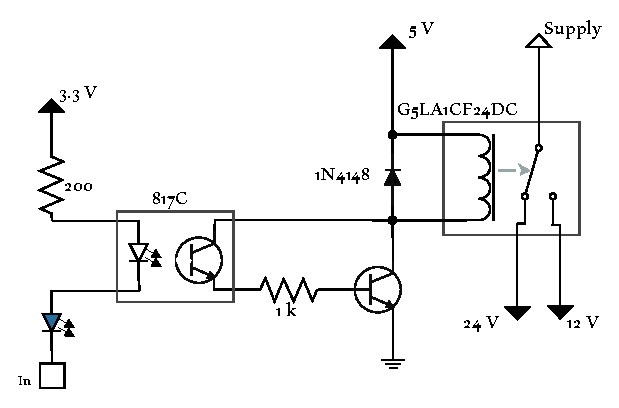
\includegraphics[width = .9\textwidth]{Sensors/relay}
		\caption{Relay circuit}
		\label{Fig:relay}
	\end{center}
\end{figure}

Summary, in the circuit represented  in (Fig.\ref{Fig:relay}) the \textit{Supply} is the voltage which is going to be provided to the electrovalves. When the \textit{In} signal is asserted, the relay is in its normal connection, son \textit{Supply} is tied to $24\ V$. On the other hand, when \textit{In} is denied relay is excited and \textit{Supply} is tied to $12\ V$.
\newpage

\begin{figure}[t]
	\centering
	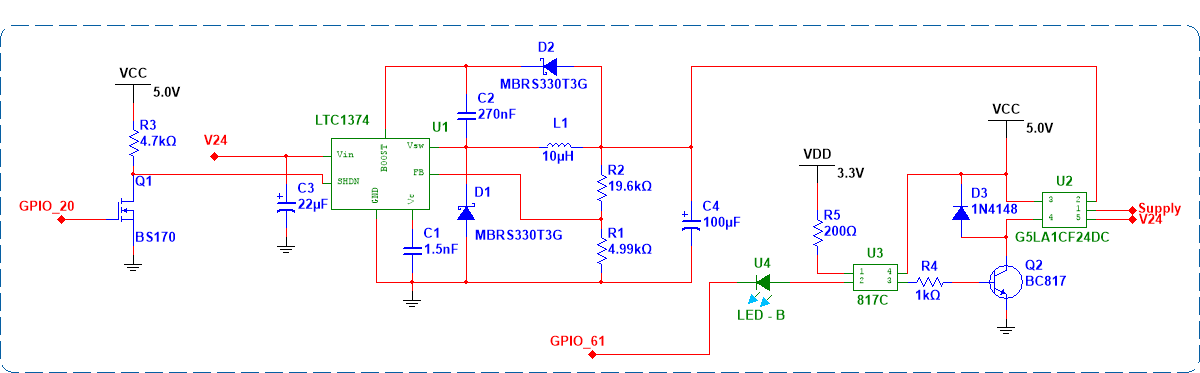
\includegraphics[width = \textwidth]{pcb/supply}
	\caption{Electrovalves Supply Circuit}
	\label{Fig:supply}
\end{figure}

The circuit in (Fig.\ref{Fig:supply}) shows the connection between \textit{DC-DC} circuit and the switching one, all of this is necessary to correctly supply the different kind of electrovalves.

